\documentclass[12pt,compress,aspectratio=169]{beamer}

\usetheme{metropolis}
\setbeamersize{text margin left=.5cm,text margin right=.5cm}
\usefonttheme{professionalfonts}

\usepackage{amsmath,bm}
\usepackage{siunitx}
%\usepackage{graphicx}
\usepackage{tikz}
\usepackage{mathpazo}
\usepackage{xcolor,colortbl}
%\usepackage{hyperref}

\setmonofont{Ubuntu Mono}
\setlength{\parskip}{0pt}
\renewcommand{\baselinestretch}{1}

\sisetup{
  number-math-rm=\mathnormal,
  per-mode=symbol
}

\title{Topic 5: Center of Mass}
\subtitle{Advanced Placement Physics}
\author[TML]{Dr.\ Timothy Leung}
\institute{Olympiads School, Toronto, ON, Canada}
\date{November 30, 2019}

\newcommand{\pic}[2]{\includegraphics[width=#1\textwidth]{#2}}
\newcommand{\mb}[1]{\ensuremath\mathbf{#1}}
\newcommand{\eq}[2]{\vspace{#1}{\Large\begin{displaymath}#2\end{displaymath}}}


\begin{document}

\begin{frame}
  \maketitle
\end{frame}



\begin{frame}{Files to Download}
  \begin{itemize}
  \item\texttt{PhysAP-05-CM-print.pdf}--The ``print version'' of this topic.
  \item\texttt{PhysAP-05-Homework.pdf}--Homework problems for Topics 4 \& 5.
  \end{itemize}
  
  \vspace{.1in}Please download/print the PDF file for the class slides before
  each class. There is no point copying notes that are already on the slides.
  Instead, focus on things that aren't necessarily on the slides. If you wish
  to print the slides, we recommend printing 4 slides per page.
\end{frame}



\begin{frame}{Center of Mass}
  Finding an object's center of mass is important, because
  \begin{itemize}
  \item Newton's laws of motion are formulated by treating an objects as point
    masses (for real-life objects, we let the forces apply to the center of
    mass)
  \item Objects can have \emph{rotational} motion in addition to
    \emph{translational} motion as well (we will examine that a bit more
    next week)
  \end{itemize}
\end{frame}



\begin{frame}{Start with a Definition}
  The \textbf{center of mass} (``CM'') is the
  \emph{weighted average of the masses in a system.} The ``system'' may be:
  \begin{itemize}
  \item A collection of individual particles (use summation to compute CM)
  \item A continuous distribution of mass with constant density (use
    integration to compute CM); in this case, CM is also the geometric center
    of the object, called the \textbf{centroid}
  \item A continuous distribution of mass with varying density (use integral to
    compute CM)
  \item If the masses are inside of a gravitational field, then the CM is also
    its \textbf{center of gravity} (``CG'')
  \end{itemize}
\end{frame}



\begin{frame}{Simple Example}
  We start with a very simple example: there are two equal masses along the
  $x$-axis. What is the center of mass of the system?
    
  \vspace{.25in}
  \begin{center}
    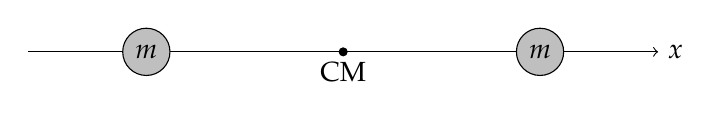
\begin{tikzpicture}
      \draw[->] (-4,0)--(4,0) node[pos=1,right]{$x$};
      \draw[fill=gray!50] (-2.5,0) circle(.3) node{$m$};
      \draw[fill=gray!50] (2.5,0)  circle(.3) node{$m$};
      \uncover<2->{
        \draw[fill=black] (0,0) circle(.05) node[below]{CM};
      }
    \end{tikzpicture}
  \end{center}
  \vspace{.2in}

  \uncover<2->{The answer is really simple: it's at the half way point between
    the two masses!}
\end{frame}

 
\begin{frame}{Things Aren't Always That Example}
  \begin{itemize}
  \item What if one of the masses are increased to $2m$?
  \item This is still not a terribly difficult problem; you can still
    \emph{guess} the right answer without knowing the equation for center of
    mass.
    
    \vspace{.25in}
    \begin{center}
      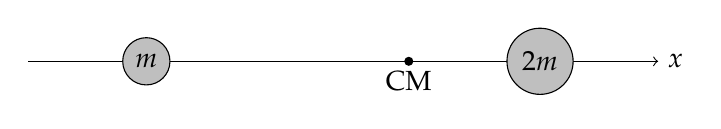
\begin{tikzpicture}
        \draw[->] (-4,0)--(4,0) node[pos=1,right]{$x$};
        \draw[fill=gray!50] (-2.5,0) circle(.3) node{$m$};
        \draw[fill=gray!50] (2.5,0) circle(.42) node{$2m$};
        \uncover<2->{
          \draw[fill=black] (.833,0) circle(.05) node[below]{CM};
        }
      \end{tikzpicture}
    \end{center}
    \vspace{.15in}

  \item<2-> The answer is still simple. The CM is no longer at the half way
    point between the two masses, but now $\frac{1}{3}$ the total distance from
    the larger masses.
  \end{itemize}
\end{frame}


\begin{frame}{Complicating Things Further}{Many Point Masses}
  If we increase the number of point masses along the $x$-axis, our problem can
  become much more complicated (although still not devastatingly so)
  \begin{center}
    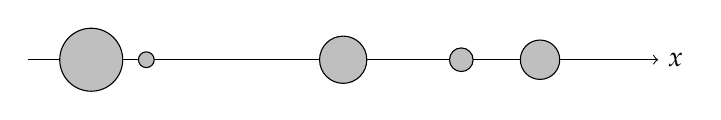
\begin{tikzpicture}
      \draw[->] (-4,0)--(4,0) node[pos=1,right]{$x$};
      \draw[fill=gray!50] (-3.2,0) circle(.4);
      \draw[fill=gray!50] (-2.5,0) circle(.1);
      \draw[fill=gray!50] (1.5,0) circle(.15);
      \draw[fill=gray!50] (0  ,0) circle(.3);
      \draw[fill=gray!50] (2.5,0) circle(.25);
    \end{tikzpicture}
  \end{center}
  
  \vspace{-.1in}Difficulties really arises when there are many masses in the
  system in 2D or 3D:
  \begin{center}
    \vspace{-.2in}
    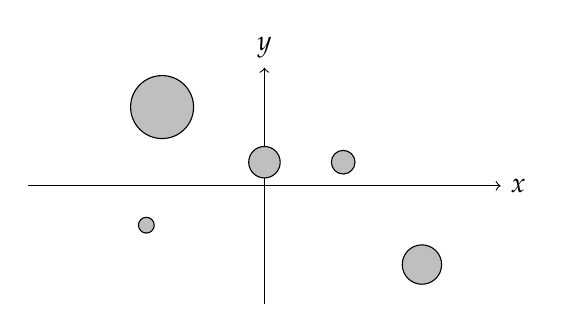
\begin{tikzpicture}
      \draw[->] (-3,0)--(3,0) node[pos=1,right]{$x$};
      \draw[->] (0,-1.5)--(0,1.5) node[pos=1,above]{$y$};
      \draw[fill=gray!50] (-1.3,1) circle(.4);
      \draw[fill=gray!50] (-1.5,-.5) circle(.1);
      \draw[fill=gray!50] (1,.3) circle(.15);
      \draw[fill=gray!50] (0,.3) circle(.2);
      \draw[fill=gray!50] (2,-1) circle(.25);
    \end{tikzpicture}
  \end{center}
\end{frame}


\begin{frame}{An Equation Helps}
  The center of mass is defined as:

  \eq{-.2in}{
    \boxed{\mb{x}_{\textrm{CM}}=\frac{\sum \mb{x}_i m_i}{\sum m_i}}
  }
  \begin{center}
    \begin{tabular}{l|c|c}
      \rowcolor{pink}
      \textbf{Quantity} & \textbf{Symbol} & \textbf{SI Unit} \\ \hline
      Position of center of mass (vector) & $\mb{x}_{\textrm{CM}}$ & \si{\metre}\\
      Position of point mass $i$ (vector) & $\mb{x}_i$ & \si{\metre}\\
      Point mass $i$ & $m_i$ & \si{\kilo\gram}\\
      Total mass & $\sum m_i$ & \si{\kilo\gram}
    \end{tabular}
  \end{center}
\end{frame}


\begin{frame}{Breaking Down Into Components}
  
  \eq{0in}{
    \boxed{\mb{x}_{\textrm{CM}}=\frac{\sum \mb{x}_i m_i}{\sum m_i}}
  }

  Position vectors have $x$, $y$ and $z$ components:
  $\mb{x}=x\hat{\bm{\imath}} + y\hat{\bm{\jmath}} + z\hat{\bm{k}}$
  which we can deal with each component individually, i.e.:

  \eq{-.2in}{
    x_{\textrm{CM}}=\frac{\sum x_i m_i}{\sum m_i}\quad\quad
    y_{\textrm{CM}}=\frac{\sum y_i m_i}{\sum m_i}\quad\quad
    z_{\textrm{CM}}=\frac{\sum z_i m_i}{\sum m_i}
  }
\end{frame}


\begin{frame}{An Example}
  \textbf{Example 1:} Consider the following masses and their coordinates
  which make up a ``discrete mass'' rigid body''
  \begin{align*}
    m_1&=\SI{5.}{\kg} &\mb{x}_1&=3\hat{\bm{\imath}}-2\hat{\bm{k}}\\
    m_2&=\SI{10.}{\kg}&\mb{x}_2&=-4\hat{\bm{\imath}}+2\hat{\bm{\jmath}}+7\hat{\bm{k}}\\
    m_3&=\SI{1.}{\kg}&\mb{x}_3&=10\hat{\bm{\imath}}-17\hat{\bm{\jmath}}+10\hat{\bm{k}}
  \end{align*}
  What are the coordinates for the center of mass of this system?
\end{frame}



\begin{frame}{Continuous Mass Distribution}
  In general, objects are not a discrete collection of point masses, but a
  continuous distribution of mass. Therefore, we take the limit of when the
  number of masses approaches $\infty$:
  
  \eq{-.15in}{
    \mb{x}_{\textrm{CM}}=\lim_{n\rightarrow\infty}
    \left(\frac{\sum_{i=1}^n \mb{x}_i m_i}{\sum_{i=1}^n m_i}\right)
  }

  This gives us an integral form of our equation:

  \eq{-.15in}{
    \boxed{\mb{x}_{\textrm{CM}}=\frac{\int\mb{x} dm}{\int dm}}
  }
\end{frame}



\begin{frame}{Densities}
  \begin{itemize}
  \item Linear density (for 1D problems)
    {\Large
      \begin{displaymath}
        \gamma=\frac{m}{L}
      \end{displaymath}
    }
  \item Surface area density (for 2D problems)
    {\Large
      \begin{displaymath}
        \sigma=\frac{m}{A}
      \end{displaymath}
    }
  \item Volume density (for 3D problems)
    {\Large
      \begin{displaymath}
        \rho=\frac{m}{V}
      \end{displaymath}
    }
  \end{itemize}
\end{frame}


\begin{frame}{An Example with Integrals}
  \begin{columns}
    \column{.65\textwidth}
    \textbf{Example 2:} A triangular plate is placed in a Cartesian coordinate
    system with two of its edges along the $x$ and $y$-axis. The length of the
    edges along the axes are $a$ and $b$ respectively. Assuming that the
    surface area density $\sigma$ is uniform, determine the coordinate of its
    center of mass.

    \column{.35\textwidth}
    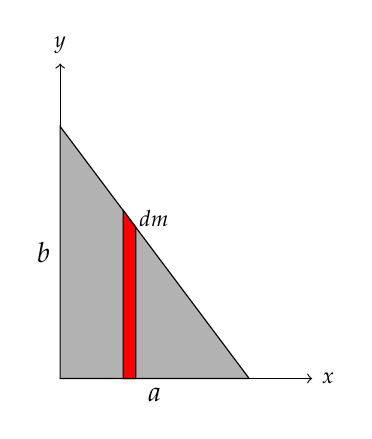
\begin{tikzpicture}[scale=.8]
      \draw[->](0,0)--(4,0) node[pos=1,right]{\footnotesize $x$};
      \draw[->](0,0)--(0,5) node[pos=1,above]{\footnotesize $y$};
      \draw[fill=gray!60](0,0)--(3,0) node[midway,below]{$a$}
      --(0,4)--cycle node[midway,left]{$b$};
      \uncover<2->{
        \draw[fill=red](1,0)--(1.2,0)--(1.2,2.4)--(1,2.67)
          node[midway,right]{\footnotesize $dm$}--cycle;
      }
    \end{tikzpicture}
  \end{columns}
\end{frame}



\begin{frame}{A Difficult Example to Try at Home}
  Not typically an AP problem, this example shows how we can use integral to
  find the center of mass for something very complicated.
  \begin{columns}
    \column{.6\textwidth}
    \textbf{Example 3:} Find the $x$-coordinate of the center of mass in the
    shape bound by the two functions shown on the right.

    \column{.4\textwidth}
    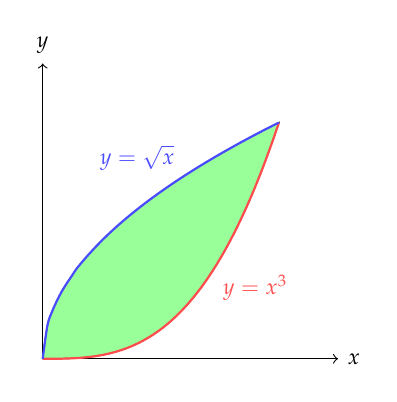
\begin{tikzpicture}[scale=3]
      \draw[->](0,0)--(1.25,0) node[pos=1,right]{\footnotesize $x$};
      \draw[->](0,0)--(0,1.25) node[pos=1,above]{\footnotesize $y$};
      \draw[fill=green!40]
      plot[smooth,samples=50,domain=0:1] (\x,{\x*\x*\x})--
      plot[smooth,samples=50,domain=1:0] (\x,{\x^(.5)});
      
      \draw[red!70,thick] plot[smooth,samples=50,domain=0:1] (\x,{\x*\x*\x});
      \draw[blue!70,thick] plot[smooth,samples=50,domain=0:1] (\x,{\x^(.5)});
      \node at (.4,.85){\textcolor{blue!70}{\footnotesize $y=\sqrt{x}$}};
      \node at (.9,.3){\textcolor{red!70}{\footnotesize $y=x^3$}};
    \end{tikzpicture}
  \end{columns}
\end{frame}



\begin{frame}{Symmetry}{There are always shortcuts!}
  \begin{itemize}
  \item Any plane of symmetry, mirror line, axis of rotation, point of inversion
    \emph{must} contain the center of mass.
  \item Caveat: only works if the density distribution is also symmetric
  \item Again: if density is uniform, CM is also geometric center (centroid)
  \end{itemize}
\end{frame}



\begin{frame}{``Negative Mass''}{A Mathematical Trick}
  \begin{itemize}
  \item Where there is a ``hole'' in the geometry, treat it as having negative
    mass density $-\sigma$ in that region.
  \item Negative masses don't exist, so this is really just a trick.
  \item\textbf{Example:} What is the center of mass of this shape?
    \begin{center}
      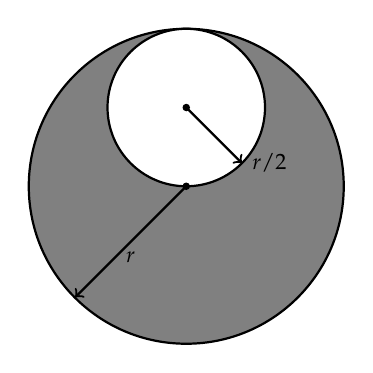
\begin{tikzpicture}
        \draw[thick,fill=gray](0,0) circle(2);
        \draw[thick,fill=white](0,1) circle(1);
        \draw[fill=black](0,0) circle(.04);
        \draw[thick,->](0,0)--(-1.41,-1.41) node[midway,below]{\footnotesize$r$};
        \draw[fill=black](0,1) circle(.04);
        \draw[thick,->](0,1)--(.707,.293) node[pos=1,right]{\footnotesize$r/2$};
      \end{tikzpicture}
    \end{center}
  \end{itemize}
\end{frame}


\begin{frame}{Negative Mass Example}
  \begin{itemize}
  \item This is how we would think of it:
    \begin{center}
      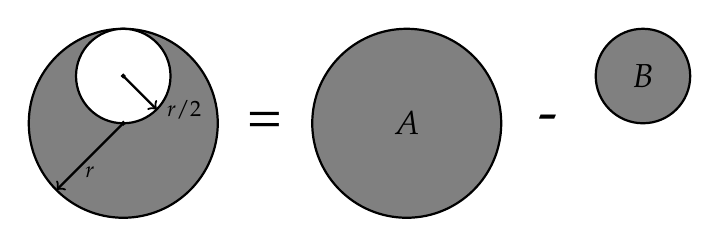
\begin{tikzpicture}[scale=.6]
        \draw[thick,fill=gray](0,0) circle(2);
        \draw[thick,fill=white](0,1) circle(1);
        \draw[fill=black](0,0) circle(.04);
        \draw[thick,->](0,0)--(-1.41,-1.41) node[midway,below]{\footnotesize$r$};
        \draw[fill=black](0,1) circle(.04);
        \draw[thick,->](0,1)--(.707,.293) node[pos=1,right]{\footnotesize$r/2$};
      
        \draw[thick,fill=gray](6,0) circle(2) node{\large$A$};
        \draw[thick,fill=gray](11,1) circle(1) node{\large$B$};
        \node at (3,0) {\huge=};
        \node at (9,0) {\huge -};
      \end{tikzpicture}
    \end{center}
  \item Let the origin of the coordinate system to located at the center of $A$
  \item Based on symmetry: $x_{\textrm{CM}}=0$; only have to find $y$-coordinate.
  \item Sum our weighted average:
    
    \vspace{-.25in}{\large
      \begin{displaymath}
        y_{\textrm{CM}}
        =\frac{\sum y_i m_i}{\sum m_i}
        =\frac{m_A(0) + m_B (r/2)}{m_A+m_B}
        =\frac{-\sigma\pi\left(r/2\right)^2(r/2)}{\sigma\pi r^2-\sigma\pi\left(r/2\right)^2}
        \uncover<2->{
          =\frac{-r}{6}
        }
      \end{displaymath}
    }
  \end{itemize}
\end{frame}



\begin{frame}{Velocity, Acceleration and Momentum}
  Take time derivative of the equation for $\mb{x}_{\textrm{CM}}$ to get the
  velocity of the CM:
    
  \eq{-.2in}{
    \mb{v}_{\textrm{CM}}=\frac{d\mb{x}_{\textrm{CM}}}{dt}
    =\frac{1}{m}\frac{d}{dt}\left(\int\mb{x}dm\right)
    =\frac{1}{m}\int\frac{d\mb{x}}{dt}dm
    =\frac{\int \mb{v}dm}{m}
  }
  
  The integral in the numerator is the sum of the momentum of all the masses in
  the system ($\mb{p}_\mathrm{net}$) which means that we have

  \eq{-.2in}{
    \mb{p}_\mathrm{net}=m\mb{v}_{\textrm{CM}}
    }

  Taking the derivative of $\mb{p}_\mathrm{net}$ relates force and acceleration
  at the CM as well:
    
  \eq{-.2in}{
    \mb{F}_\mathrm{net}=\frac{d\mb{p}_\mathrm{net}}{dt}
    =m\frac{d\mb{v}_{\textrm{CM}}}{dt}=m\mb{a}_{\textrm{CM}}
  }
\end{frame}


%\begin{frame}{What This All Means}
%  \begin{itemize}
%  \item Newton was right all along by treating all objects as point masses
%    located at the CM
%  \end{itemize}
%\end{frame}

\end{document}
